\chapter{Filterverschleiß}
\label{ch:Filterverschleiß}
Ausgehend von der Auswahl der Filter im vorherigen Kapitel \ref{ch:auswahl} wird nun das Phänomen Filterverschleiß näher erläutert. Es folgt zunächst ein allgemeiner Teil zu Verschleiß an Tiefenfiltern allgemein. Weiterhin werden die gewählten Filter in diesem Kontext detaillierter beschrieben.
\section{Auftretende Verschleißerscheinungen}
\label{sec:auftr}
    Grundsätzlich sind Filterschäden Versagensarten, die einen zweckmäßigen Betrieb unmöglich machen. Allgemein als Filterbruch bezeichnet, bedeutet dies ein mechanisches Versagen in unterschiedlicher Form. Mögliche Beispiele sind Risse im Filtermedium und Ablösungen des Filtermediums vom Rahmen, wodurch kontanimierte Luft durch den Spalt am Filter vorbei gelangt. Ursachen hierfür sind \cite{filterfail}:
    \begin{itemize}
        \item Mechanische Eigenschaften / Verschleiß
        \item Chemische Korrosion
        \item Thermische Korrosion
        \item Durchdringung / Verstopfung
        \item Konstruktionsfehler
    \end{itemize}
    Filterschäden können auch von durch den Luftstrom beschleunigten Objekten, wie z.B. Metallsplitter, über ballistische oder Schneidwirkung das Filtermaterial zerstören. 
    Bei den üblichen Strömungsgeschwindigkeiten in \ac{lta}'s ist diese Ursache allerdings unwahrscheinlich. Die Ursachen lassen sich insgesamt auf Korrosion und Staubbeladung im weiteren Sinne zurückführen. In Folge verschlechtern sich die mechanischen Eigenschaften von Filtermedium und Dichtung. Bei gleichbleibenden Volumenstrom, also Nutzen des Filters erhöht die Staubbeladung die Last auf den Filtern, und kann somit auch als eine Verschleißart angesehen werden. Außerdem kann die Art des Staubes die unterschiedlichen Korrosionsarten beschleunigen.
\begin{figure}[H]
    \begin{center}
%
       \subfigure[Bersten in Folge von Druck]{%
           \label{fi:schaden_berst}
           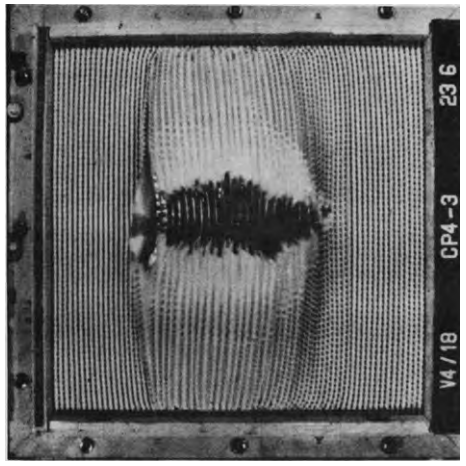
\includegraphics[width=0.5\textwidth]{images/schaden_berst.png}
       }%
       \subfigure[Versagen einzelner Faltentaschen]{%
          \label{fi:schaden_falten}
          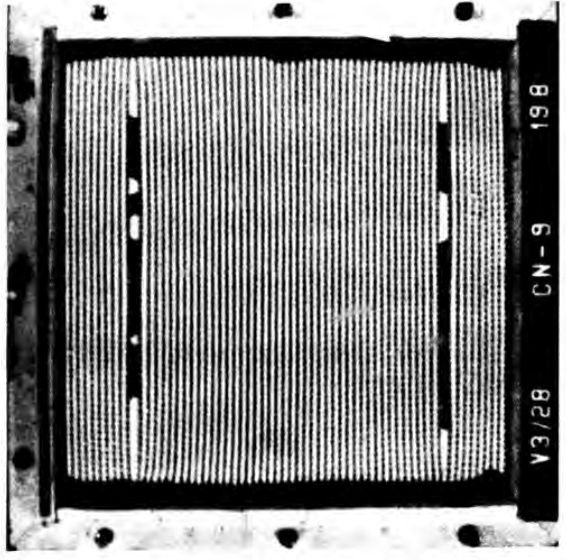
\includegraphics[width=0.5\textwidth]{images/schaden_falten.png}
       }\\ %  ------- End of the first row ----------------------%
       \subfigure[Schaden durch Seperatorkanten in Folge des Anschwellens des Filtermediums]{%
           \label{fi:schaden_seperator}
           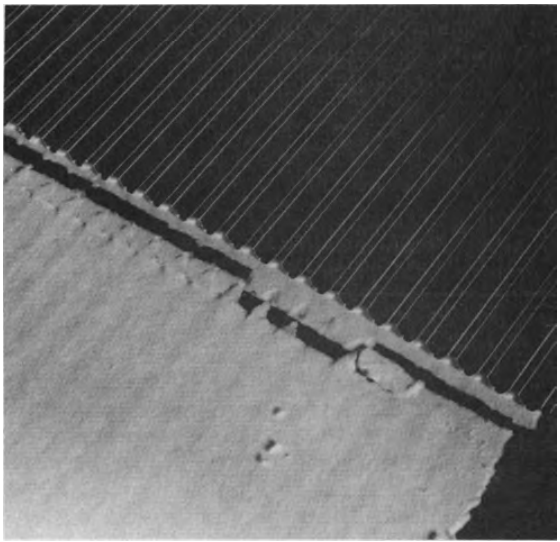
\includegraphics[width=0.5\textwidth]{images/schaden_seperator.png}
       }%
       \subfigure[Schaden an Dichtung/Verklebung zum Rahmen]{%
           \label{fi:schaden_rand}
           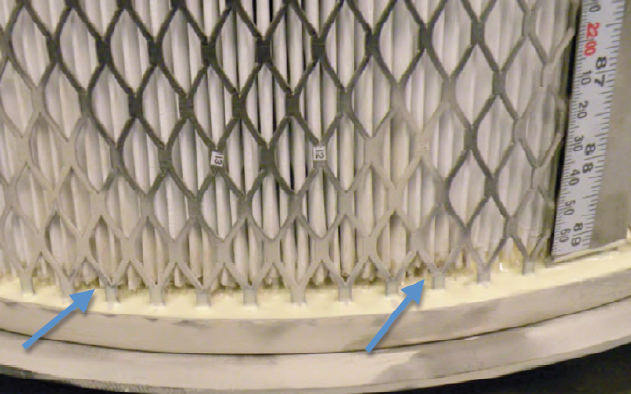
\includegraphics[width=0.5\textwidth]{images/schaden_rand.png}
       }\\%

%
   \end{center}
   \caption{%
       Unterschiedliche Schadenarten an Filtern. Abb. \ref{fi:schaden_berst} bis \ref{fi:schaden_seperator} nach Rüdinger \cite{rudinger}; Abb. \ref{fi:schaden_rand} nach Bergmann \cite{hepa}
    }%
  \label{fig:schadensarten}
\end{figure}
\section{Filterkollaps}
    Im Falle der Faltenstruktur bei leistungsfähigen Filtern ist der Kollaps der Faltenstruktur (siehe Abb. \ref{fi:kollaps}) ursächlich für lokale Differenzdruckspitzen, welche zum mechanischen Versagen des Filtermediums führen. Derartige Strukturen zur Oberflächenmaximierung werden häufig bei diversen Filterarten eingesetzt. Die in Folge des Kollaps verringerte Filteroberfläche verursacht eine weitere Erhöhung der Druckdifferenz durch den Filter, was den Effekt kaskadenartig verstärkt.\cite{hepa} Bergman \cite{hepa} hat zur Abschätzung des Filterkollaps eine Berechnungsgrundlage vorgeschlagen, welche auf der ARbeit von Rüdinger zu den auftretenden Spannungen im Filtermedium \cite{rudinger} aufbaut.
    \begin{figure}[H]
        \begin{center}
            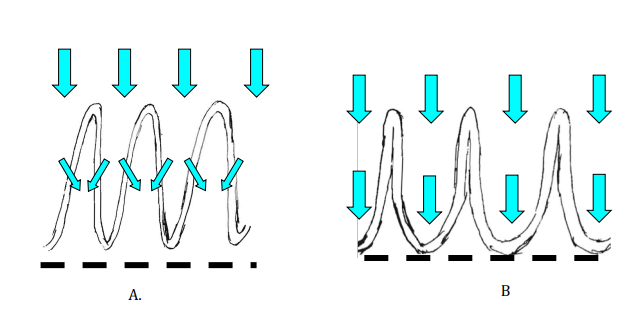
\includegraphics[width=\linewidth]{images/kollaps.png}
            \caption[Filterkollaps]{Prinzipskizze mit (A) intaktem Filter, und (B) Filter mit zunehmenden Kollaps \cite{hepa}}
            \label{fi:kollaps}
        \end{center}
    \end{figure}
    Dieser Kollaps kann nur eintreten, wenn die Steifigkeit der Struktur nicht mehr ausreicht, um der Verformung durch den Differenzdruck zu widerstehen. Aus diesem Grund werden z.B. Abstandshalter aus unterschiedlichen Werkstoffen in den Filtern verbaut (siehe Abb. \ref{fi:seperator}) und/oder Versteifungsprägungen (siehe Abb. \ref{fi:versteifung}) oder andere Versteifungsstrategien in die Filtermatten eingearbeitet.
    Im Fall von Filtern, die in Lüftungsanlagen von Gebäuden eingesetzt werden, führen hohe Temperaturen und Feuchtigkeit zu einer Herabsetzung der Steifigkeit des Filtermediums.\cite{hepa} Hierbei ist auch hervorzuheben, dass die zunehmende Filtratbelastung, Korrosion ausgenommen, keinen Einfluss auf die mechanischen Eigenschaften der Filterfasern, und somit auch nicht auf die Steifigkeit, hat. 
    \begin{figure}[H]
        \begin{center}
    %
           \subfigure[Versteifungsprägungen \cite{giffin}]{%
               \label{fi:versteifung}
               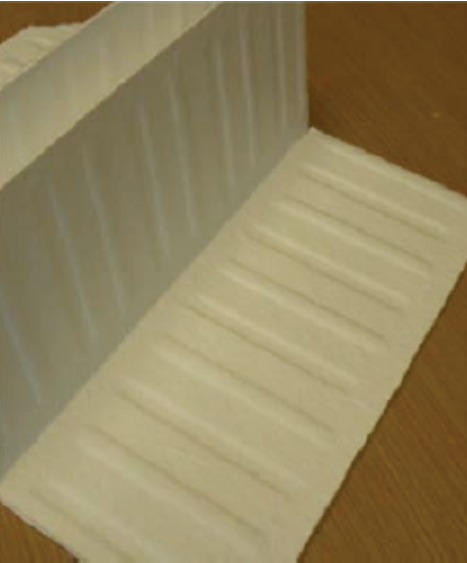
\includegraphics[width=0.5\textwidth]{images/versteifungen.png}
           }%
           \subfigure[Abstandshalter (Seperator) \cite{seperator}]{%
              \label{fi:seperator}
              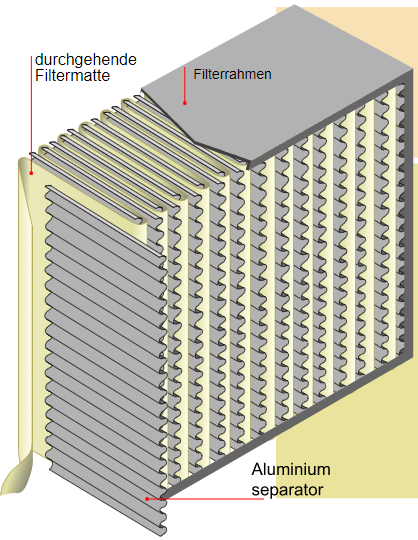
\includegraphics[width=0.5\textwidth]{images/seperator.png}
           }\\ %  ------- End of the first row ----------------------%
    
    %
       \end{center}
       \caption{%
           Gegenmaßnahmen Filterkollaps
        }%
      \label{fig:subfigures}
    \end{figure}
    Die in Datenblättern von Filtern angegebene maximale Druckdifferenz beschreibt den Wert, bei dem abgeschiedener Staub mitgerissen werden kann, der Werkstoff des Filtermediums versagt unter dieser Last normalerweise noch nicht (vgl. Datenblätter empf./max. Druckdifferenz).
    Mit Hinblick auf auftrende Schadensbilder unterscheiden sich Tiefenfilter also hauptsächlich hinsichtlich der Struktur des Filtermediums. Eine Unterscheidung zwischen Filtermedien mit Faltenstruktur, und solchen ohne Faltenstruktur (Filtervliese, Matten etc.) macht dahingehend Sinn, das bei solchen ohne Faltenstruktur keine Effekte auftreten, welche die effektive Filteroberfläche verringern. Hier sind die Säume bzw. Dichtungen typische Schwachstellen. Daher sind für die Analyse von Filterschäden grundsätzlich Kenntnisse über die mechanischen Eigenschaften des Filtermediums nötig. Um diese an Filtermedien zu erfassen, wird für Materialen mit Berstdruck unter 600 kPa  eine Prüfung nach DIN ISO 2758\cite{2758} empfohlen. Ansonsten sind keine einheitlichen Prüfverfahren für den Berstdruck von Filtermedien beschrieben. Das Prüfverfahren, auch Mullen-Burst-Strenght Test genannt, beinhaltet die Einspannung des Prüflings, und eine Beaufschlagung des Prüflings mit hydraulischem Druck auf ein elastisches Membran. Diese Prüfung berücksichtigt jedoch nicht die spätere Geometrie des Filtermediums (Faltenstruktur), was eine gesonderte Prüfung im Kontext Filterkollaps erforderlich macht. \\
    Eine weitere, typische Schwachstelle sind die Dichtungen bzw. Aufnahmen zwischen Filtermedium und Rahmen des Filterelements. Diese unterscheiden sich hinsichtlich Verschleiß und Schadensbilder ebenso je nach Bauform und Werkstoff. Während bei metallischen Rahmen sicherlich die Feuchte treibender Faktor für eine Korrosion ist, sind für Kunststoffe a priori zusätzlich Temperaturschwankungen ungünstig. Weil somit für die unterschiedlichen Dichtungsformen der Verschleiß kaum allgemein darstellbar ist wären insbesondere für die Untersuchung dieser Verschleißformen anwendungsnahe Versuche nötig.
    \section{Identifikation geeigneter Messgrößen}
    \label{sec:ident_mess}
    Die Auswahl der Messgrößen ist abhängig vom Anlagenaufbau, bzw. Art der Steuerung. Bei entsprechender Klimatechnik, sind für die Überwachung nachgelagerter Filter z.B. keine Messungen der Feuchte nötig, da hier von konstanten Bedingungen ausgegangen werden kann. Eine Überwachung der Strömungsgeschwindigkeiten und/oder Differenzdrücke kann ebenfalls bereits implementiert sein. \newline
    Die Standzeit der Filter selbst ist primär abhängig von Speichervermögen, Filtrat(Staub) und Volumenstrom. Da das Ziel der Überwachung die maximale Ausnutzung des Speichervermögens, bei gleicher oder besserer Sicherheit ist, sind also Daten bezüglich Staubzusammensetzung und -Last unabdingbar. Die unterschiedlichen Messgrößen müssen also ausreichen, um zu erkennen, wann eine ungünstige Kombination aus hoher Druckdifferenz (vollem Speicher) und Umweltfaktoren auftritt, die die mechanischen Eigenschaften des Filtermediums überschreiten. \newline
    Hierzu sind folgende Messgrößen zu erfassen: Druckdifferenz am jew. Filter, Volumenstrom (evtl. auch rechnerischer Wert aus z.B. Ventilatordrehzahl), Temperatur, Feuchtigkeit und Staublast/-zusammensetzung der Außenluft. Eine relativ geringe Abtastrate von einem Wert pro Minute ist hierbei als ausreichend zu bewerten. Allerdings können evtl. Druckstöße durch z.B. Wechsel der Fahrweise,  Windstöße usw. bei zunehmender Abnutzung interessant werden. Dies erfordert gesonderte Versuche zur Ermittlung der Größenordnung der in Folge auftretenden Druckschwankungen, und eine erneute Evaluation der Abtastraten.
    \section{Einfluss der Regelungsart}
    \label{sec:regelungsart}
    Die Regelung von \ac{lta}'s lässt sich in die Regelung des Volumenstroms gegen Druckwiderstände etc. und die Regelung in Bezug auf den Bedarf (s. Abb. \ref{fi:regelungsarten}) trennen. Erstere erfolgt hierbei vorwiegend auf Feldebene an \ac{ddc} Stationen, wobei in modernen Anlagen zunehmend Bussysteme wie KNX, LONWorks oder BACnet eingesetzt werden, was eine zentrale Regelung über z.B. dedizierte Server oder moderne \ac{sps} ermöglicht. Die Nutzung von Bussystemen verringert außerdem den Verkabelungsaufwand, was bei der Ausrüstung von Gebäuden hinsichtlich Planung und Installation Kosten einspart. \newline
    Soll die vorgestellte Lösung auch auf die Abluftseite der Anlage adaptiert werden, wird eine Regelung nach IDA-C5 bzw. C6 erforderlich, da andererseits keine Informationen über die tatsächlich auftrende Staublast im Gebäude gewonnen werden können. Für die Zuluftseite sind laufende, detaillierte Messungen der Luftqualität unter verschiedenen Wetterlagen eines möglichst langen Zeitraums erforderlich.
    Grundsätzlich bedingen bedarfsgesteuerte Regelungsarten einen niedrigeren Filterverschleiß, da die Filter außerhalb der vollen Nutzung nicht unnötig mit Staub beaufschlagt werden. Bei derart geregelten \ac{lta}'s ist daher eine höhre Standzeit der Filter zu erwarten. Eine Bewertung der Schimmelbildung oder anderer Biobelastung in Folge von Zyklen ohne ausreichende Lüftung der geschlossenen Systeme müsste individuell erfolgen. Beispielsweise könnte, in Folge von durchgängiger Home-Office Regelungen während einer Pandemie, eine zusätzliche Steuerungsschleife erforderlich sein, um dieser Verschleißart gerecht zu werden.
    Sicher ist jedoch, dass der Volumenstrom nicht nur Einfluss auf die Staublast pro Zeiteinheit, mit der der jeweilige Filter beaufschlagt wird, sondern auch auf die Wirkung der unterschiedlichen Filtereffekte hat. Daher muss der Volumenstrom auch, zeitvariant oder konstant geregelt, in ein Vorhersagemodell zum Filterverschleiß einfließen. Dies erfordert folglich auch entsprechende Messtechnik oder eine Berechnung aus geeigneten Prozessgrößen, wie z.B. Ventilatordrehzahlen.

    \section{Einfluss von Umgebungsbedingungen}
    \label{sec:umweltbed}
    Unterschiedliche Umgebungsbedingungen haben eine erheblichen Einfluss auf die Filterlast. Das Schadstoffgehalte, und somit Fraktionsanteile und Menge des Staubes, natürlichen, und anthropogenen Schankungen unterliegen, ist hinreichend bekannt.
    Folglich ist auch die Lage der Anlage von Bedeutung, denn in der Nähe von z.B. Schwerindustrie, vielbefahrenen Straßen und Agrarflächen ist die Staubbelastung signifikant höher. Bei der Auslegung von Anlagen wird daher die Außenluft (\ac{oda}) nach DIN EN 16798 \cite{16798} klassifiziert (s. Abb. \ref{fi:oda_class}).
    \begin{figure}[H]
        \begin{center}
            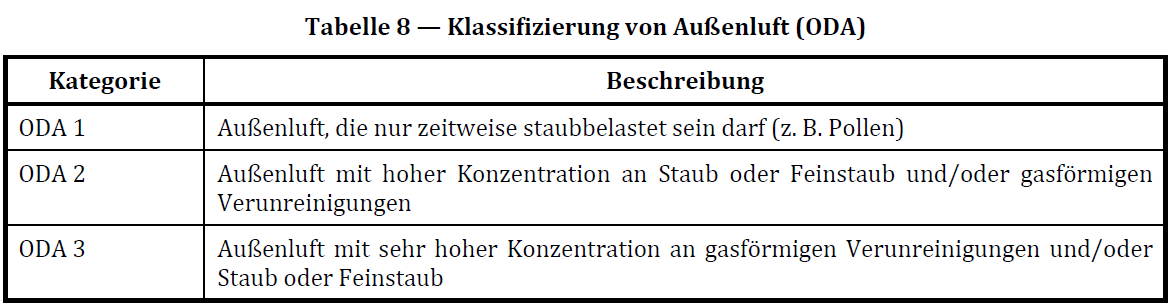
\includegraphics[width=\linewidth]{images/oda_class.png}
            \caption[Klassifizierung von Außenluft]{Klassifizierungen der Außenluft nach DIN EN 16798-3 \cite{16798} }
            \label{fi:oda_class}
        \end{center}
    \end{figure} 
    Bei ODA 1 werden alle WHO-Grenzwerte unterschritten; Bei ODA 2 liegen alle Luftschadstoffwerte unter dem anderthalbfachen Grenzwert; liegt ein Wert über dem anderthalbfachen Grenzwert gilt ODA 3. Die Außenluft fließt somit nur als Mittel- bzw. Maximalwert über einen längeren Zeitraum in die Auslegung. Wie bereits angemerkt, wäre für eine prädiktive Überwachung allerdings eine Schnittstelle zu z.B. Messstellen des Umweltbundesamtes für Echtzeitdaten, oder eine Erweiterung des Modells um eine Korrelation zwischen Wetterdaten und Luftschadstoffmengen sinnvoll, um die tatsächliche Staublast in eine Prognose einzubeziehen. Beispiele hierfür sind saisonaler Pollenflug, Smogbildung bei ungünstigen Wetterlagen, oder erhöhtes Verkehrsauskommen an bestimmten Wochentagen. Für das Simulationsmodell zur Datenerzeugung werden diese tages- und jahreszeitlichen Schwankungen jedoch nicht in diesem Detailgrad berücksichtigt.
    Desweiteren hat die Temperatur und Luftfeuchte Einfluss auf die Sorptionsisotherme der Filtermedien. Beispielsweise wird, bei höheren Außentemperaturen und hoher Luftfeuchte, speziell an Außenfiltern mehr Feuchtigkeit kondensieren und auf das Filtermedium einwirken. Wetterdaten wirken sich außerdem auf die in Kap. \ref{sec:auftr} beschriebenen Korrosionsarten aus.


 